\section{JTAG Data Register for User}
\label{sec:JTAGDataForUSer}

In the JTAG TAP controller of mmRISC-1, a 32bit USER register is added to the standard specification as shown in Table \ref{tb:JTAGDATAFORUSER}. The 5bit address of the USER register is 0x0f which is specified by the IR register. As shown in Figure \ref{fig:JTAGCHAIN}, if the USER register is selected, the TAP controller captures 32bit width input signal \seqsplit{JTAG\_DR\_USER\_IN} into the JTAG shift chain at CAPTURE\_DR state, and updates the USER register by copying from the JTAG shift chain at UPDATE\_DR state. The contents of the USER register are connected to 32bit width output signal \seqsplit{JTAG\_DR\_USER\_OUT}. \\


\begin{table}[H]
    \begin{adjustbox}{scale={1}{1}}
    \textsf{
    \begin{tabular}{|L{2cm}{1.5cm}{t}|L{6cm}{4cm}{t}|L{9cm}{7cm}{t}|}
        \hline
        %-------------------------------------
        \rowcolor{LightPurple}
        \textbf{Address} &
        \textbf{Name} &
        \textbf{Description}
        \nextRow \hline
        %-------------------------------------
        0x00 & BYPASS & JTAG recommends this encoding
        \nextRow \hline
        %-------------------------------------
        0x01 & IDCODE & JTAG recommends this encoding
        \nextRow \hline
        %-------------------------------------
        \rowcolor{lime}
        0x0F & USER	& For User (mmRISC-1 original)
        \nextRow \hline
        %-------------------------------------
        0x10 & DTMCS & For Debugging
        \nextRow \hline
        %-------------------------------------
        0x11 & DMI & For Debugging
        \nextRow \hline
        %-------------------------------------
        0x12 & Reserved (BYPASS) & Reserved for future RISC-V debugging
        \nextRow \hline
        %-------------------------------------
        0x13 & Reserved (BYPASS) & Reserved for future RISC-V debugging
        \nextRow \hline
        %-------------------------------------
        0x14 & Reserved (BYPASS) & Reserved for future RISC-V debugging
        \nextRow \hline
        %-------------------------------------
        0x15 & Reserved (BYPASS) & Reserved for future RISC-V debugging
        \nextRow \hline
        %-------------------------------------
        0x16 & Reserved (BYPASS) & Reserved for future RISC-V debugging
        \nextRow \hline
        %-------------------------------------
        0x17 & Reserved (BYPASS) & Reserved for future RISC-V debugging
        \nextRow \hline
        %-------------------------------------        
        0x1F & BYPASS & JTAG requires this encoding
        \nextRow \hline
        %-------------------------------------
    \end{tabular}
    }
    \end{adjustbox}
    \caption{JTAG Data Register for User}
    \label{tb:JTAGDATAFORUSER}
\end{table}



\begin{figure}[H]
    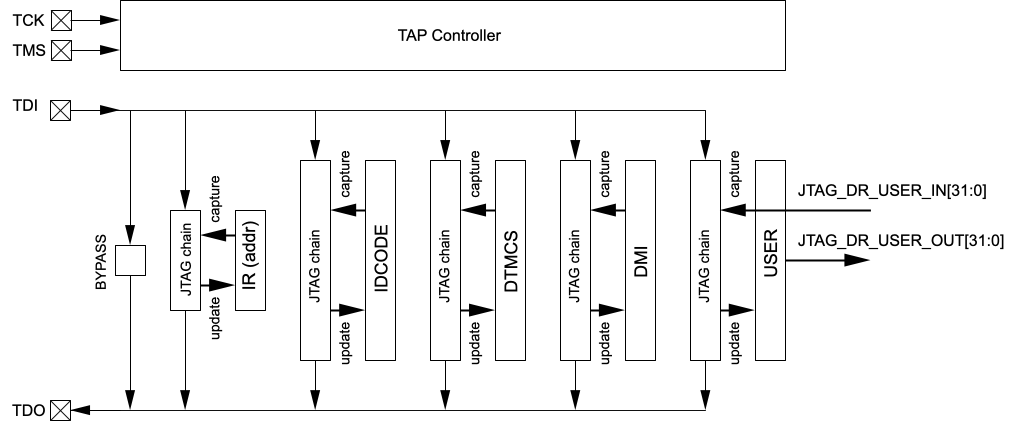
\includegraphics[width=1.00\columnwidth]{./Figure/JTAG_Chain.png}
    \caption{Block Diagram of JTAG Chain in mmRISC-1}
    \label{fig:JTAGCHAIN}
\end{figure}


